\documentclass{article}
\usepackage[a4paper, margin=2.5cm]{geometry} 
\usepackage{ctex}        
\usepackage{graphicx}    
\usepackage{amsmath}     
\usepackage{amssymb}     
\usepackage{fancyhdr}   
\usepackage{titlesec}   
\usepackage{listings}    
\usepackage{xcolor}
\usepackage{titlesec}
\usepackage{array}
\usepackage{float}
\usepackage{placeins}
\usepackage{tikz}
\usetikzlibrary{positioning}


\titleformat{\section}{\centering\Large\bfseries}{\thesection}{1em}{}

\title{{\bf 人工智能导论 Lab-2 实验报告}}
\author{褚砺耘 2023012471 \\ 致理-信计31}
\date{\today}

\begin{document}

\maketitle

\section{实验环境}

\begin{itemize}
    \item 操作系统:macOS Sonoma 14.6.1
    \item Python版本:Python 3.12.4
    \item CPU:Apple M3
\end{itemize}

\section{CNN 模型}

\subsection{数据预处理}

对于给定的数据集 train.txt, test.txt, validation.txt 首先加载数据,得到原始句子 + 标签的数据格式,
然后对原始句子进行分词,并构建词表 \texttt{word2id:\{"<PAD>":0, "<UNK>":1, ...\}},然后根据词表将
句子转换为 ID 序列。我们设置 max\_len = 60, 将所有序列设置为该长度(超出截断, 不足补0)。然后根据 Word2Vec 将每个词转换为
长度为 50 的向量,并剔除无法识别的词语(OOV words), 构建成 max\_len $\times 50$ 的词向量矩阵。同时我们同样需要把
代表情感正向与负向表示为二维张量:$[1,0]$ 与 $[0,1]$.

\subsection{模型结构图}

\begin{figure}[h]
    \centering
    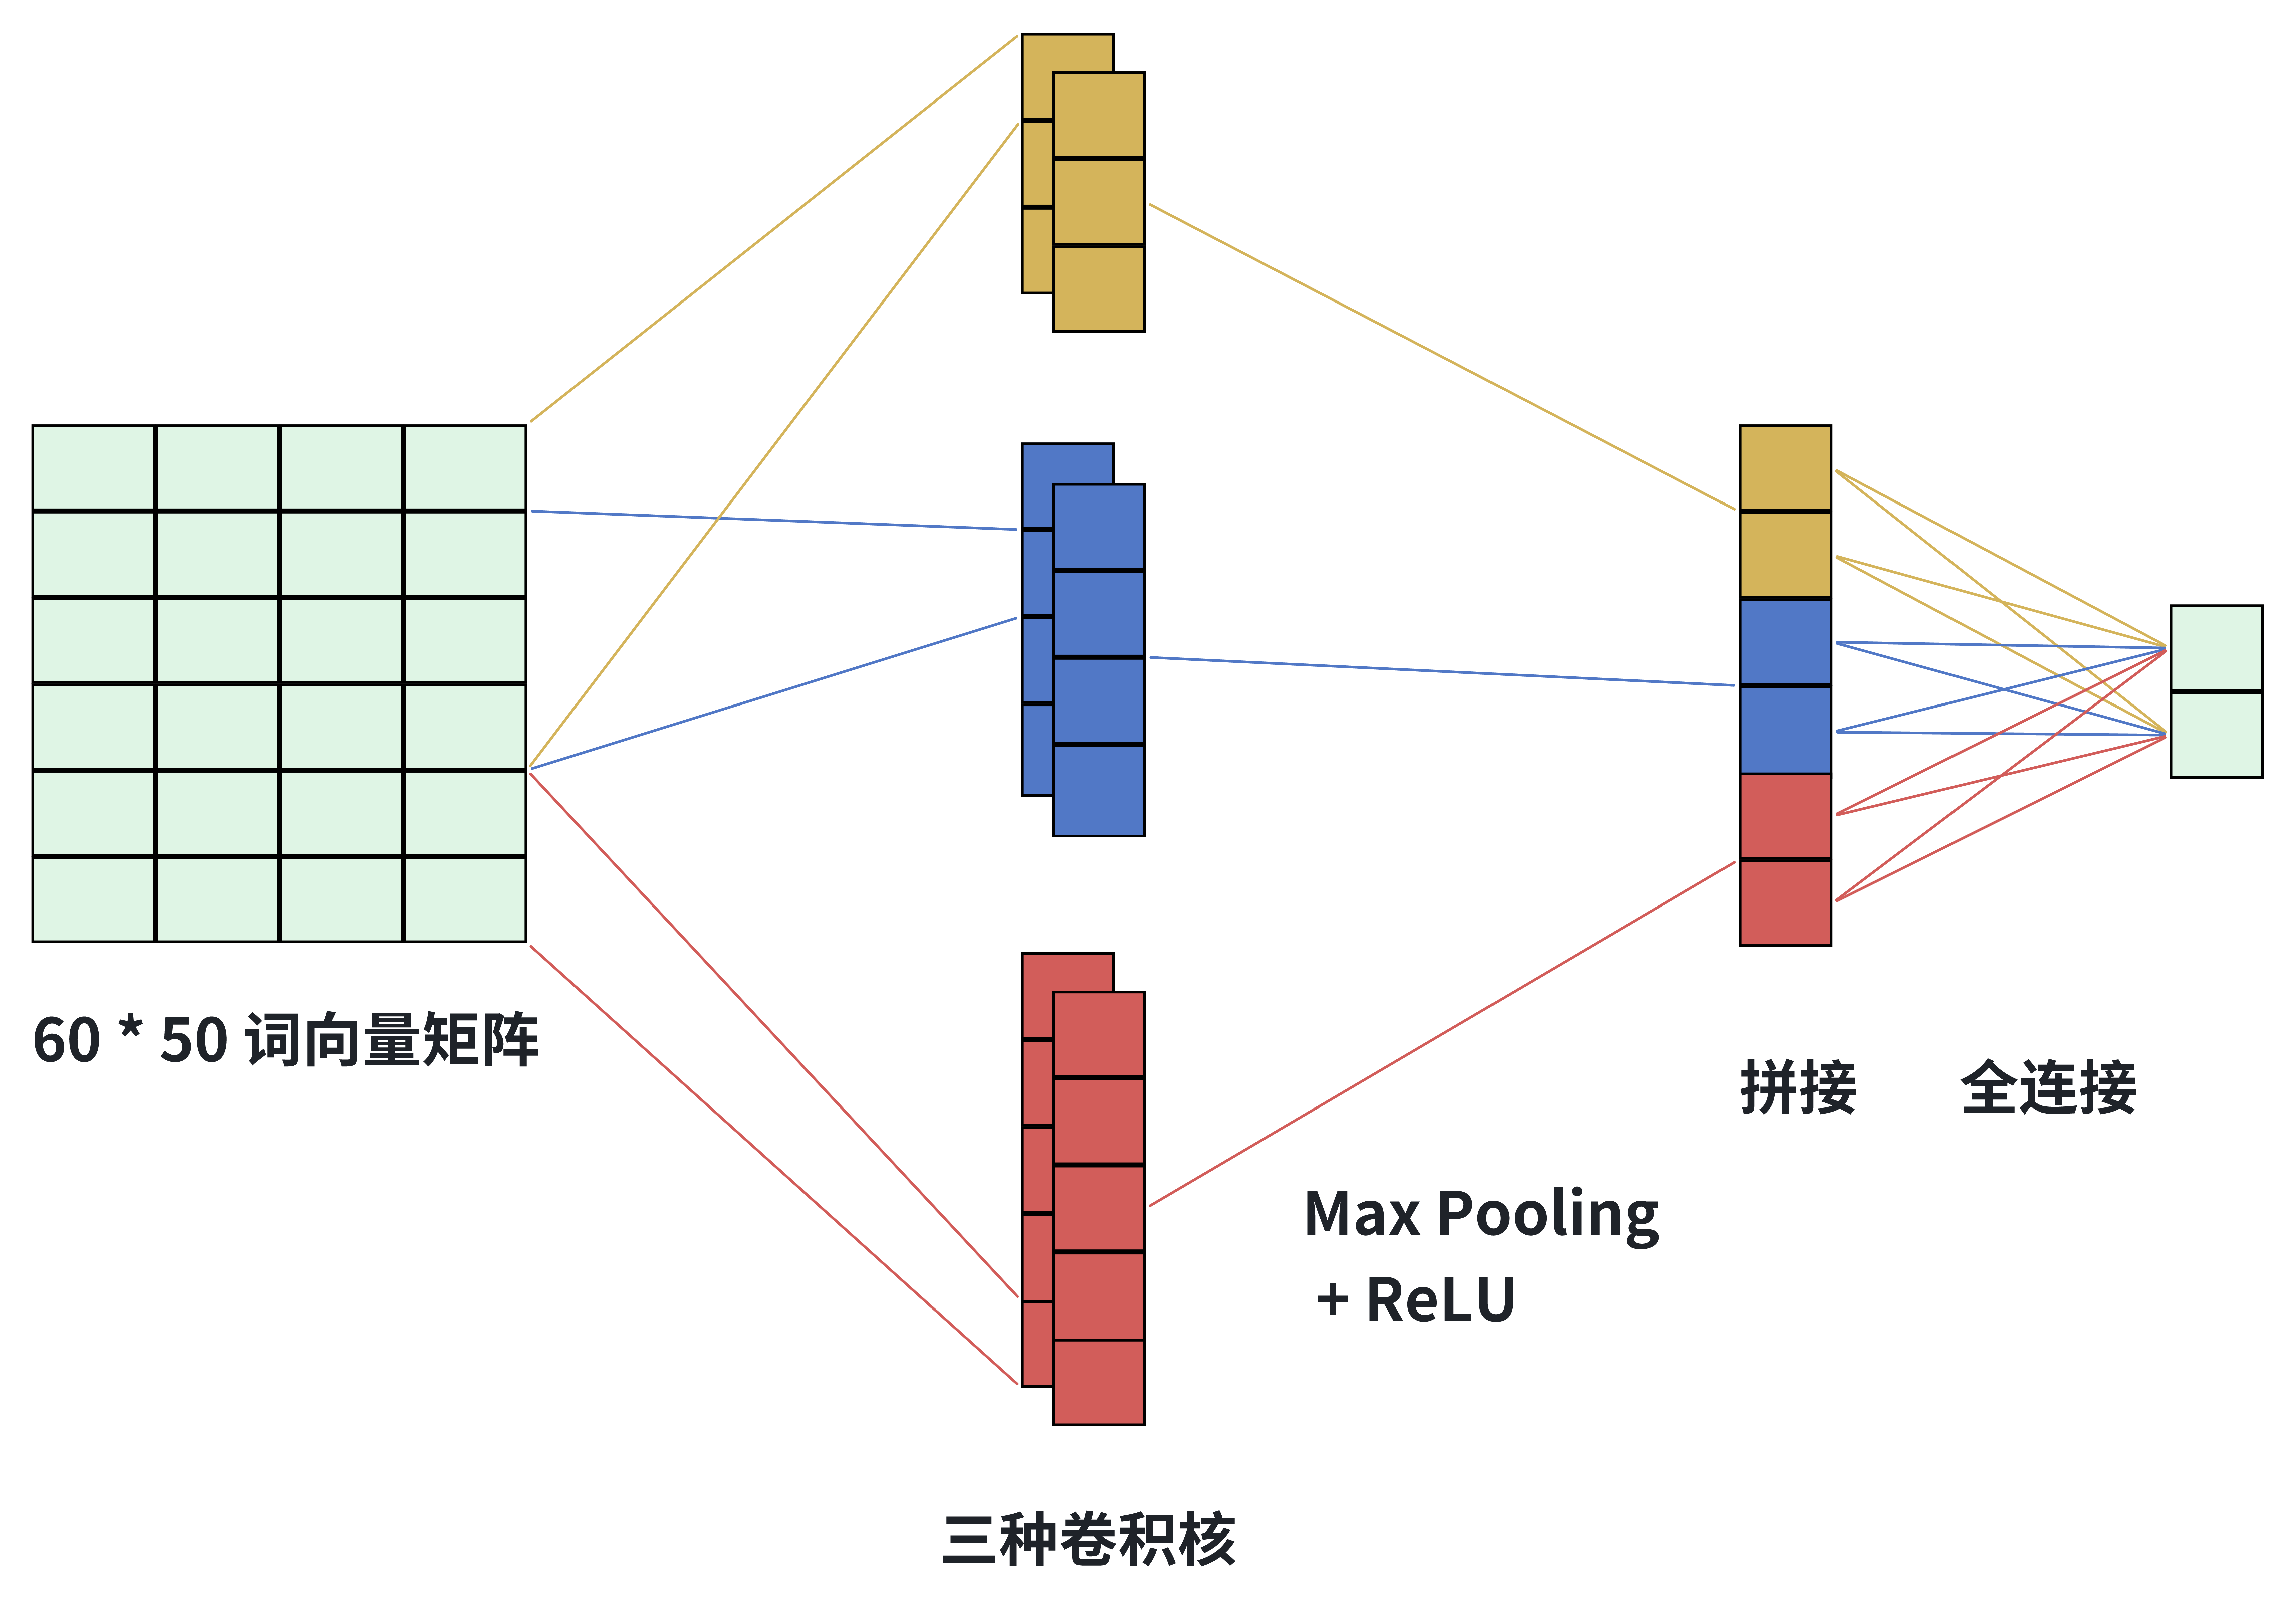
\includegraphics[width=0.6\textwidth]{img/cnn.png}
\end{figure}

\FloatBarrier

\subsection{流程分析}

\begin{enumerate}
    \item 输入句子:
        \begin{itemize}
            \item 原始句子被转换成 max\_len 长度的序列
            \item 经过词嵌入层变成 shape 为 [batch\_size, max\_len, 50] 的张量
        \end{itemize}
    \item 卷积层:
        \begin{itemize}
            \item 使用 3 个卷积核尺寸: 3, 4, 5
            \item 每种卷积核使用 num\_filiters = 100 个
            \item 卷积核在“句子维度”上滑动,卷积的是局部的 n-gram
        \end{itemize}
    \item 激活 + 最大池化:
        \begin{itemize}
            \item 每个 filter 经过 ReLU 激活后进行最大池化,池化后的结果是 1 个数
            \item 每个 kerner\_size 会输出 100 维的特征向量
        \end{itemize}
    \item 拼接:
        \begin{itemize}
            \item 将三个卷积核输出的结果拼接起来,得到300维向量。
        \end{itemize}
    \item 全联接层 
        \begin{itemize}
            \item 送入具有两个神经元的全连接层,输出 [batch\_size, 2] 的logits向量。使用Softmax激活函数。
        \end{itemize}
    \item 损失函数:使用交叉熵计算loss。
\end{enumerate}

\subsection{实验结果}
超参数如下:

\begin{table}[H]  
    \centering        
    \begin{tabular}{|c|c|}
    \hline
    {\bf 超参数} & {\bf 数值} \\
    \hline
    epoch & 10  \\
    \hline
    batch\_size & 128  \\
    \hline
    learning\_rate & 2e-3  \\
    \hline
    kernel\_sizes & 100 \\
    \hline
    max\_len & 60 \\
    \hline
    \end{tabular}
\end{table}

train、val accuracy:
\begin{figure}[h]
    \centering
    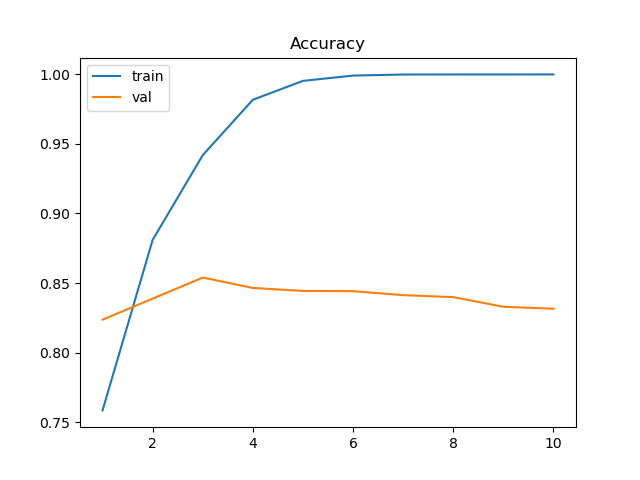
\includegraphics[width=0.6\textwidth]{../results/cnn_acc.png}
\end{figure}

\FloatBarrier

train、val loss:
\begin{figure}[h]
    \centering
    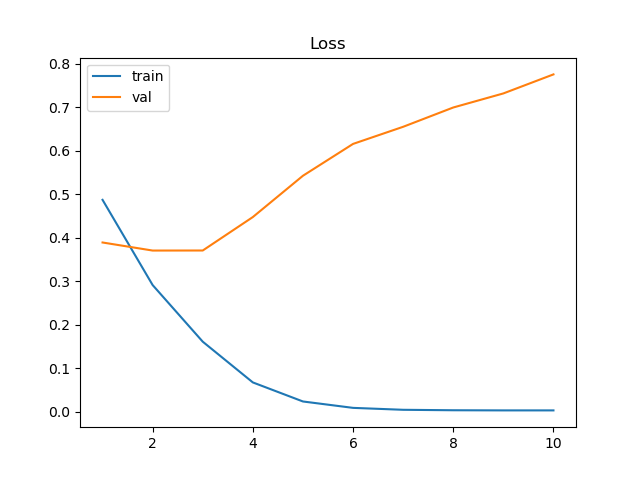
\includegraphics[width=0.6\textwidth]{../results/cnn_loss.png}
\end{figure}

\FloatBarrier

val F1:
\begin{figure}[htbp]
    \centering
    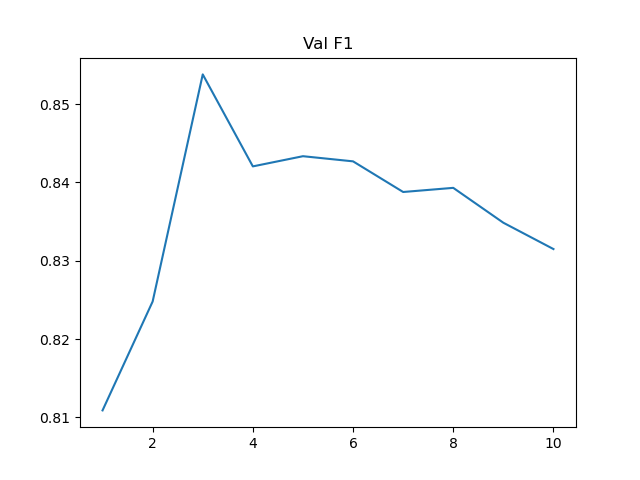
\includegraphics[width=0.6\textwidth]{../results/cnn_f1.png}
\end{figure}

\FloatBarrier

在test set上的表现为:

\begin{table}[H]
    \centering
    \begin{tabular}{|c|c|}
        \hline 
        {\bf 指标} & {\bf 数值} \\
        \hline
        Loss & 0.6261 \\
        \hline 
        Accuracy & 0.8645 \\
        \hline
        F1 & 0.8619 \\
        \hline
    \end{tabular}
\end{table}

\section{RNN-LSTM}

\subsection{数据预处理}
同上 CNN 模型的数据预处理过程。

\subsection{模型结构图}

\begin{figure}[htbp]
    \centering
    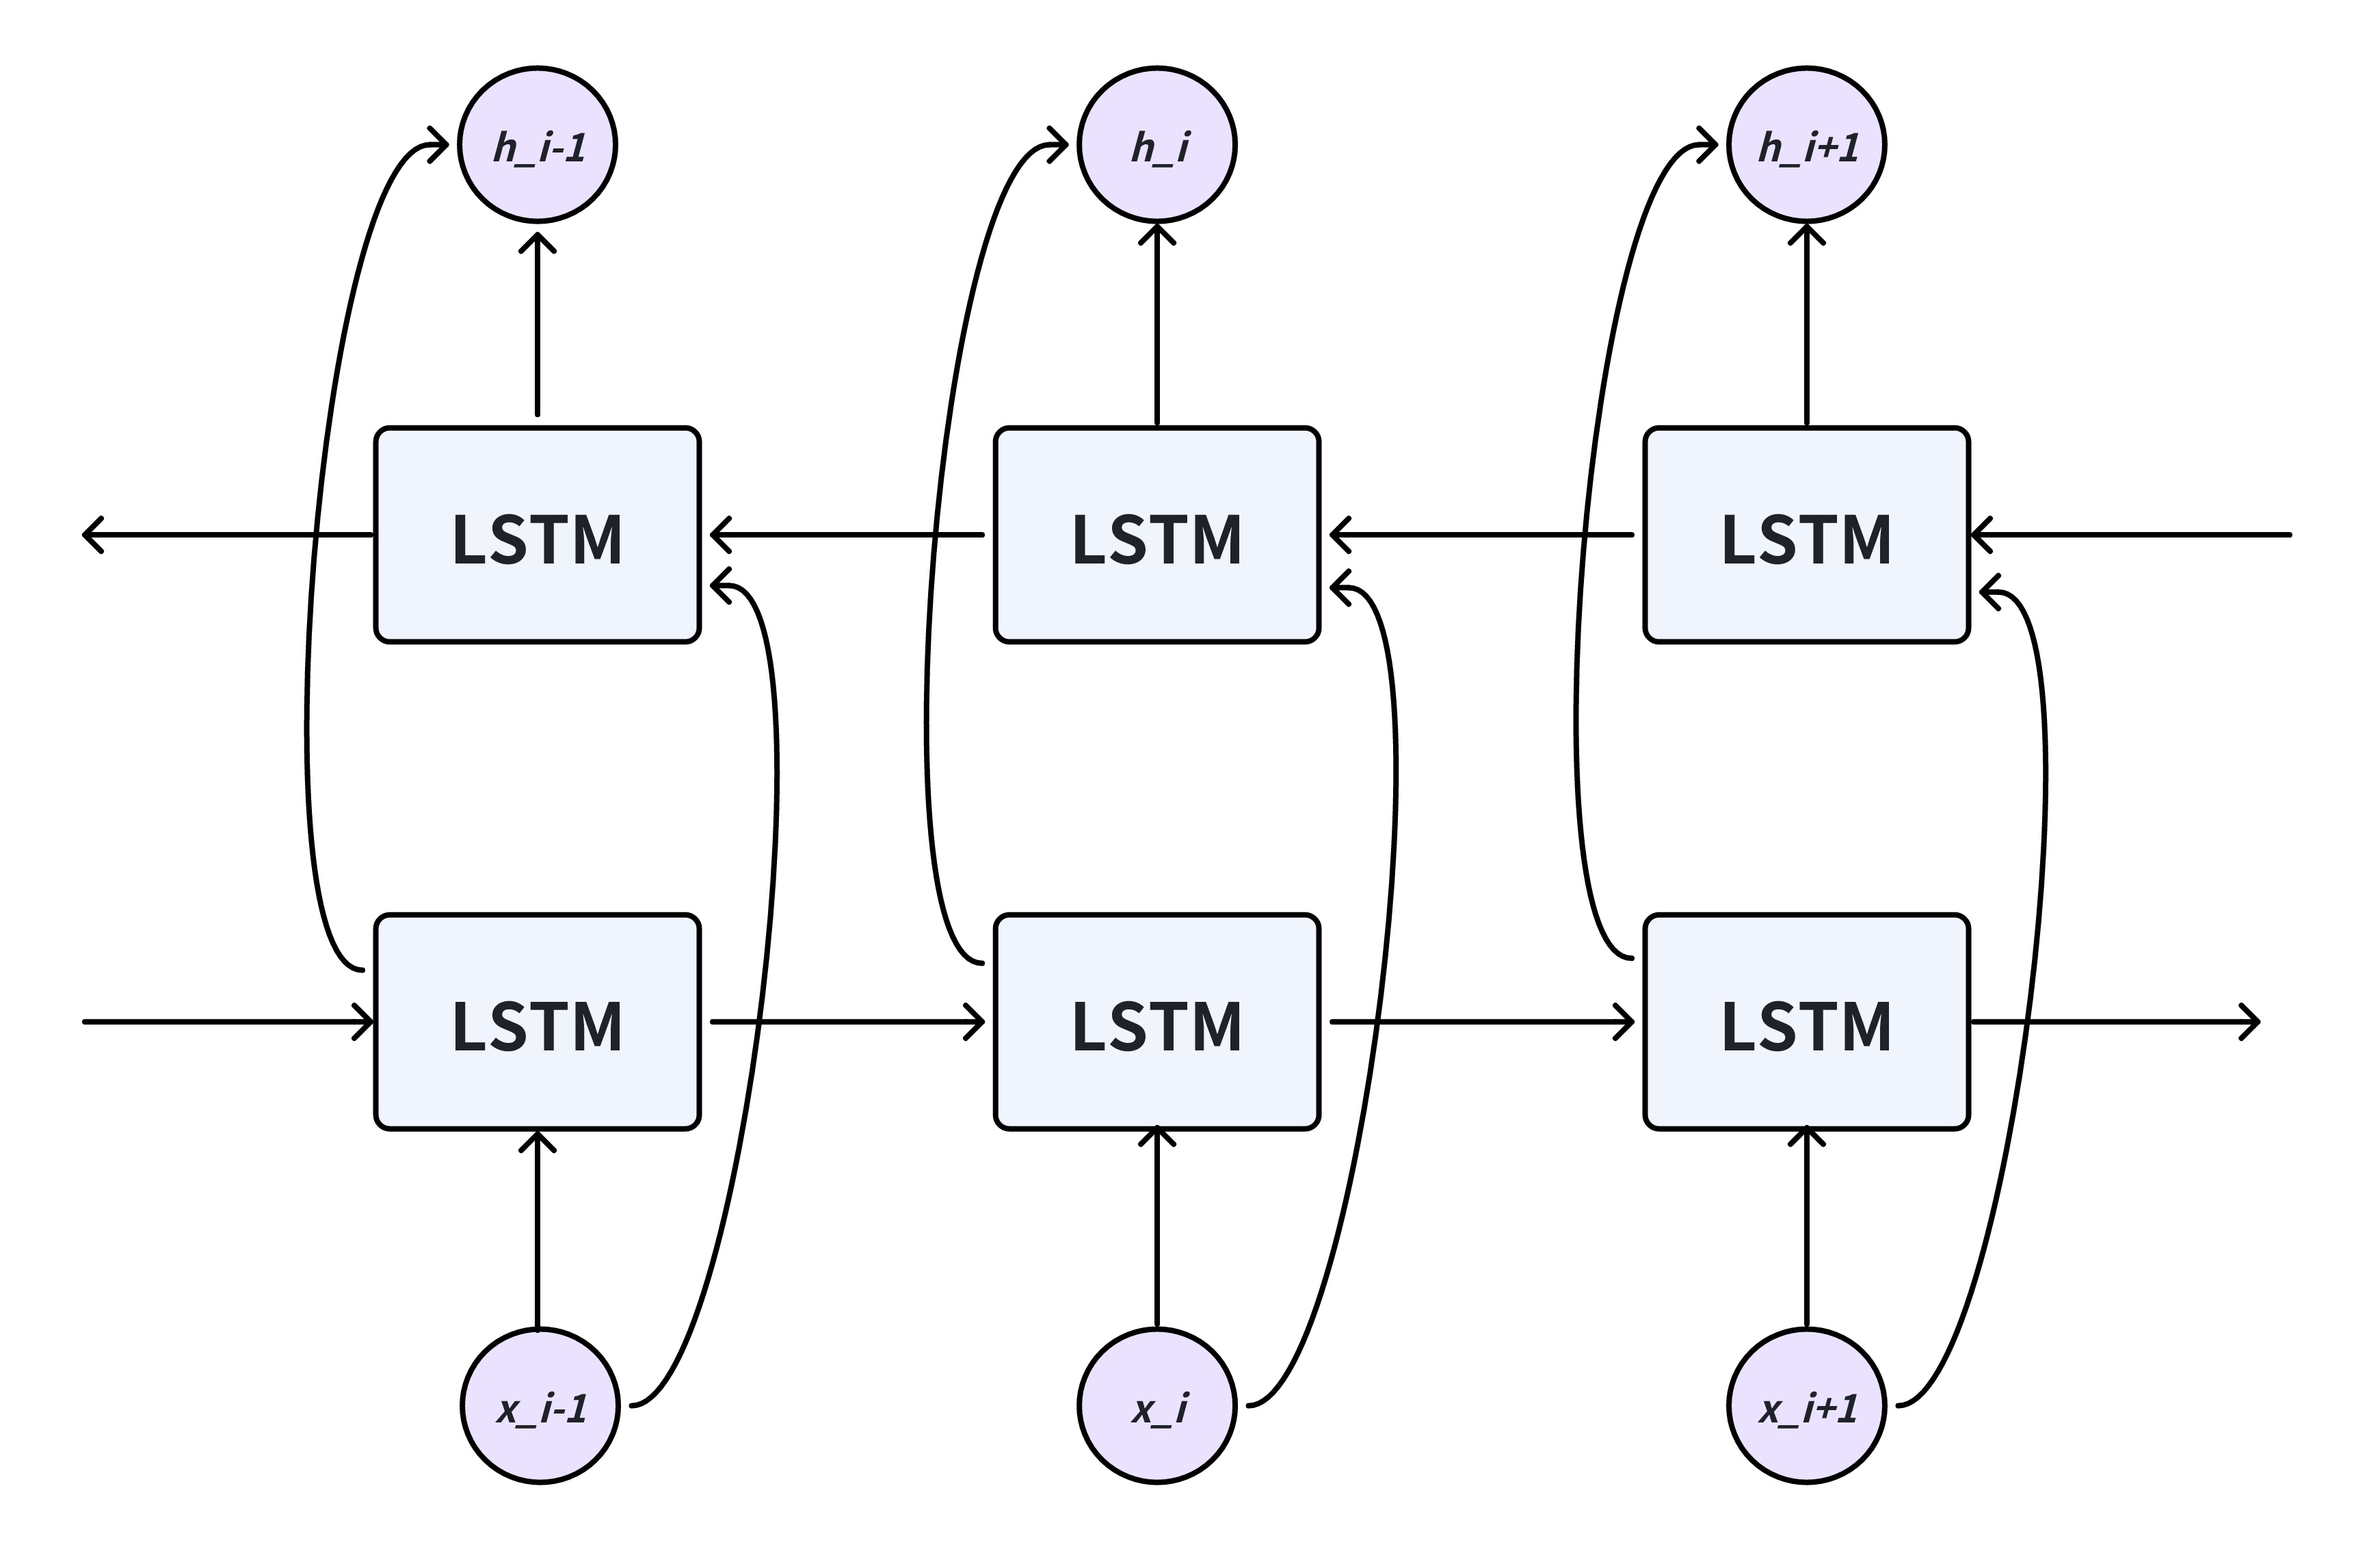
\includegraphics[width=0.6\textwidth]{img/lstm.png}
\end{figure}

如果是单向lstm, 则只有向前传播的模块。

\FloatBarrier

\begin{figure}[htbp]
    \centering
    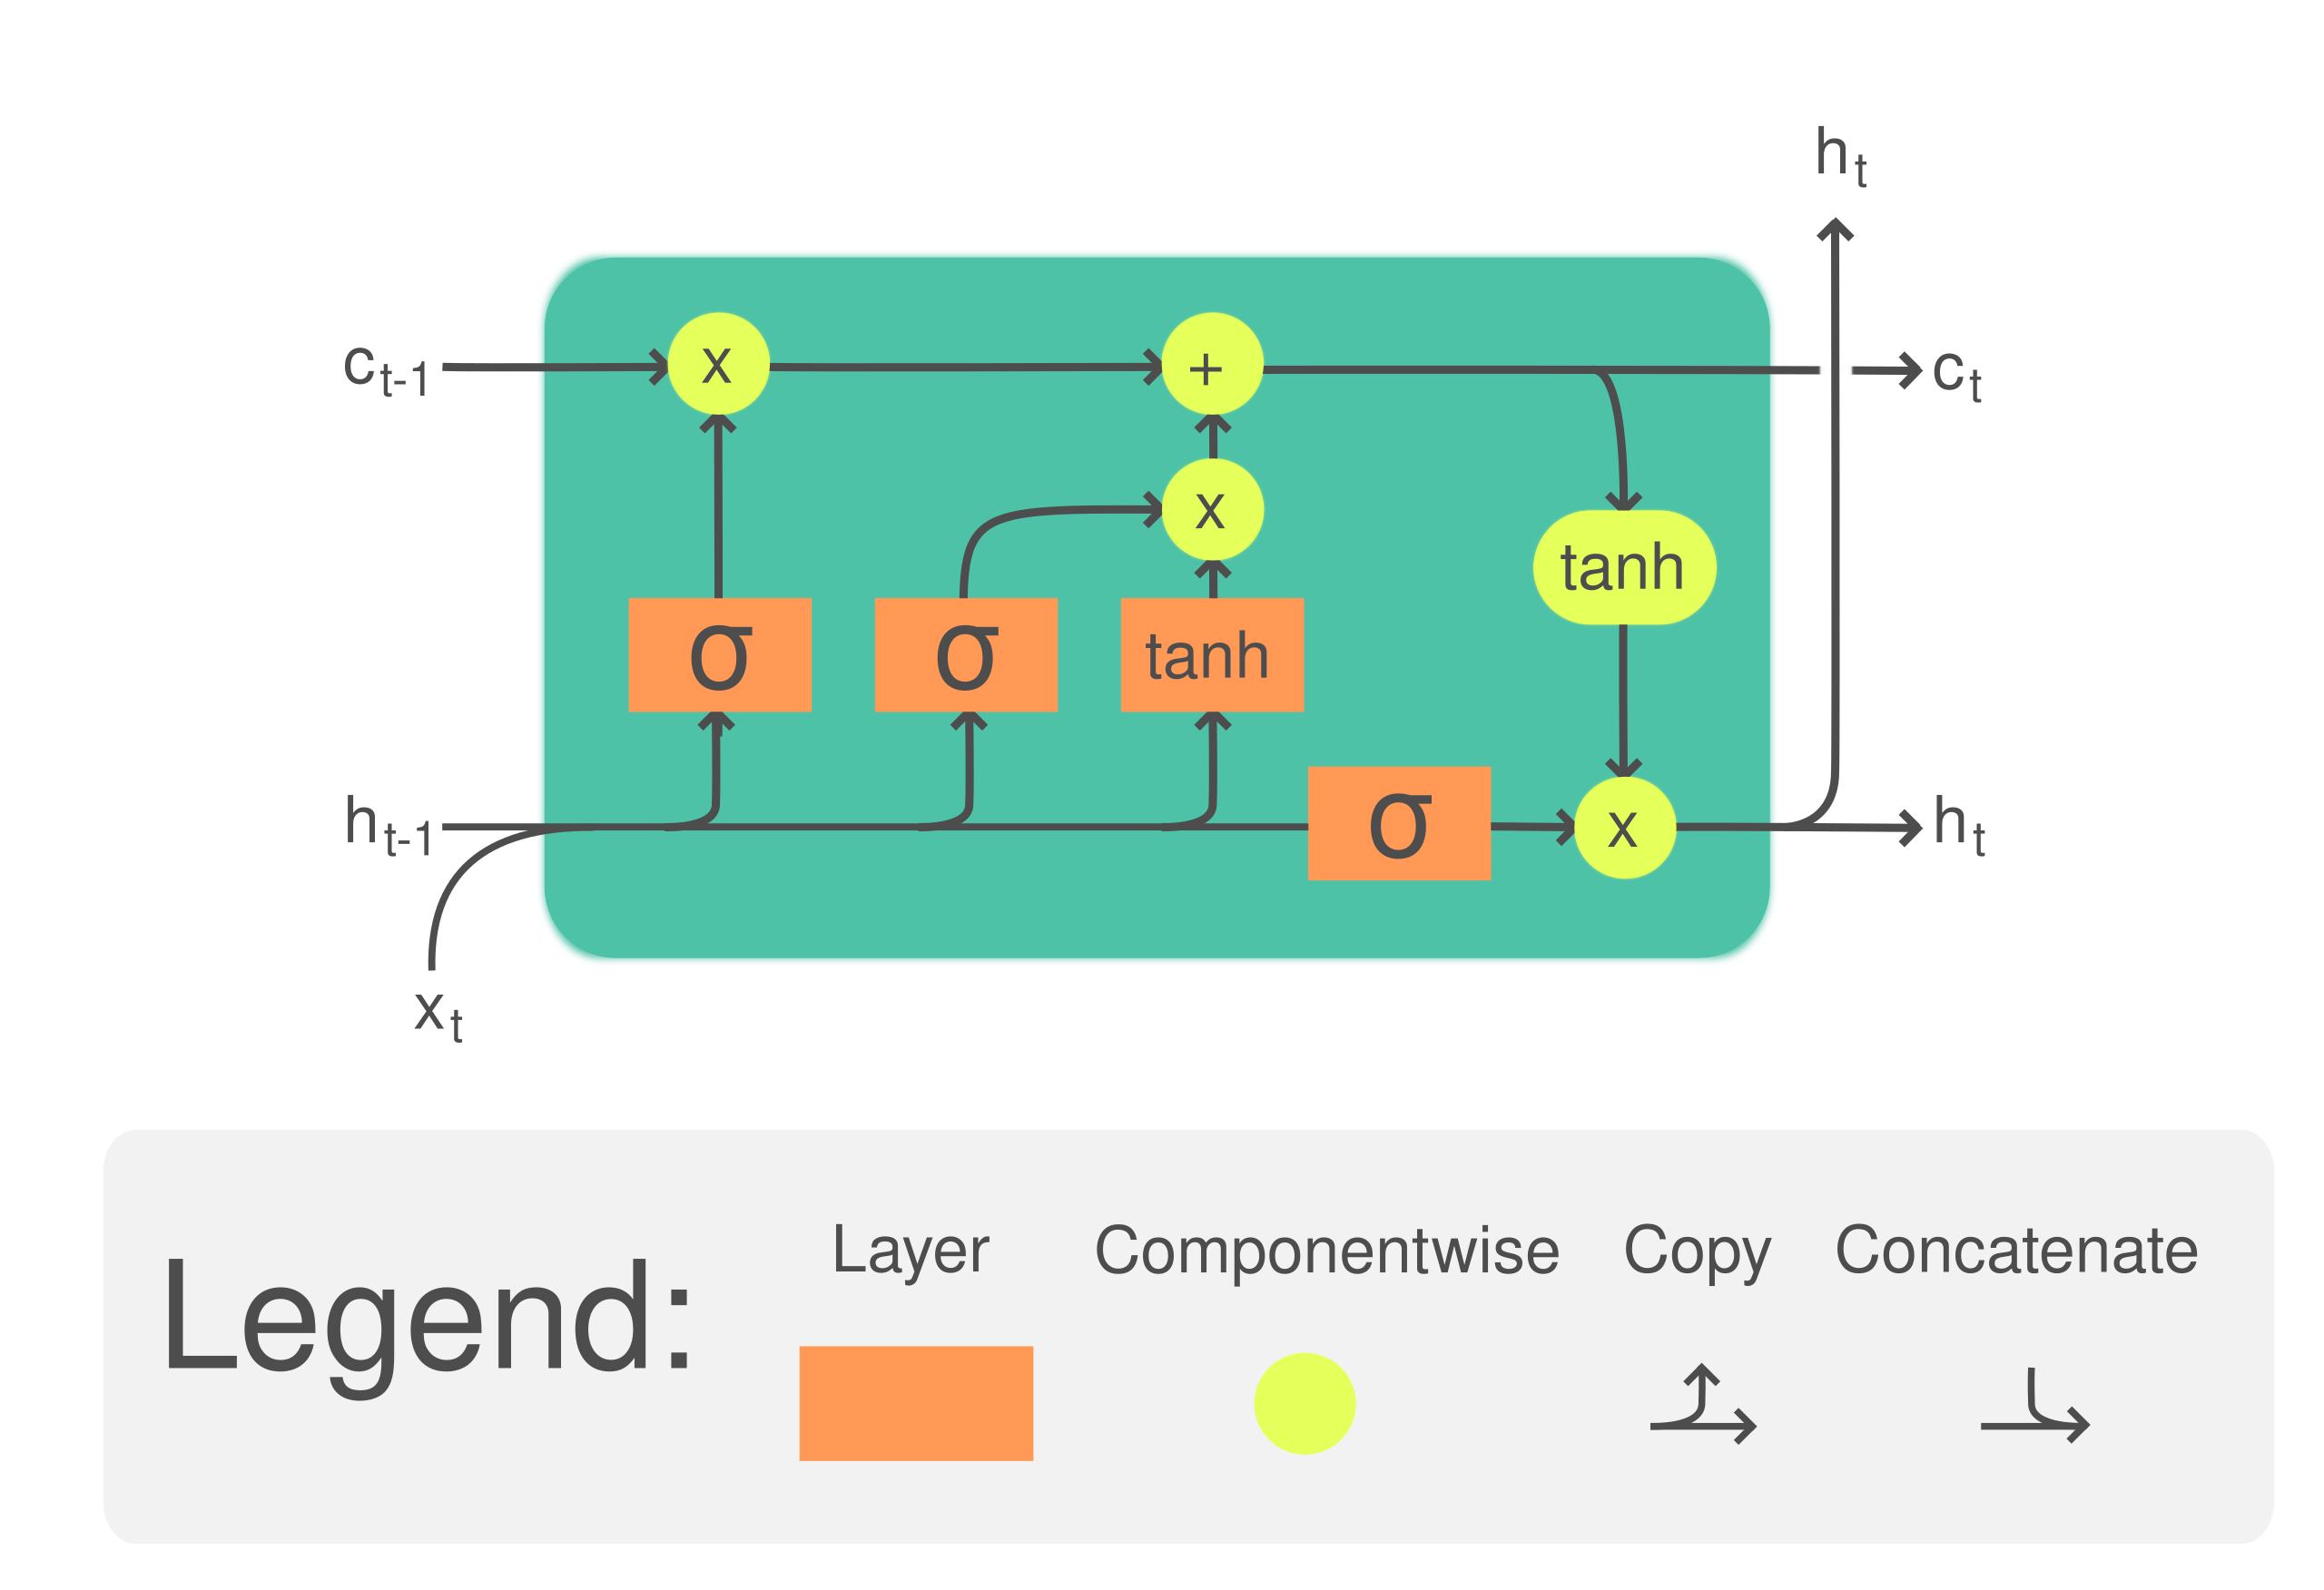
\includegraphics[width=0.6\textwidth]{img/LSTM_Cell.svg.png}
\end{figure}

\FloatBarrier

\subsection{流程分析}

\begin{enumerate}
    \item 输入句子:
        \begin{itemize}
            \item 原始句子被转换成 max\_len 长度的序列
            \item 经过词嵌入层变成 shape 为 [batch\_size, max\_len, 50] 的张量
        \end{itemize}
    \item 输入LSTM模块:
        \begin{itemize}
            \item 分别采用单向和双向的 LSTM 模型, num\_layers = 1,hidden\_size = 128  
        \end{itemize}
    \item 输入全连接层:
        \begin{itemize}
            \item 对于单向 LSTM, 直接对正向结果使用 $128\times 2$的全连接层
            \item 对于双向 LSTM, 将正向结果和反向结果拼接后使用 $256\times 2$的全连接层
        \end{itemize}
    \item Softmax激活、计算交叉熵损失、反向传播、更新。
\end{enumerate}

\subsection{实验结果}
超参数如下:

\begin{table}[H]  
    \centering        
    \begin{tabular}{|c|c|}
    \hline
    {\bf 超参数} & {\bf 数值} \\
    \hline
    epoch & 10  \\
    \hline
    batch\_size & 128  \\
    \hline
    learning\_rate & 2e-3  \\
    \hline
    hidden\_size & 128 \\
    \hline
    num\_layers & 1 \\
    \hline
    max\_len & 60 \\
    \hline
    \end{tabular}
\end{table}

我们绘出单向 LSTM 的结果图像。train、val accuracy:
\begin{figure}[h]
    \centering
    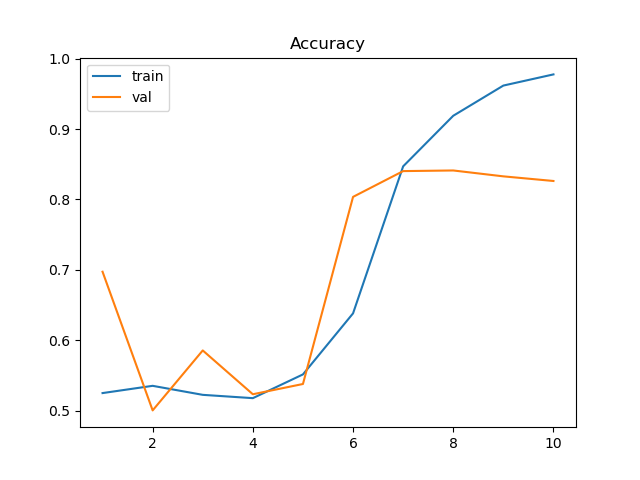
\includegraphics[width=0.6\textwidth]{../results/lstm_acc.png}
\end{figure}

\FloatBarrier

train、val loss:
\begin{figure}[h]
    \centering
    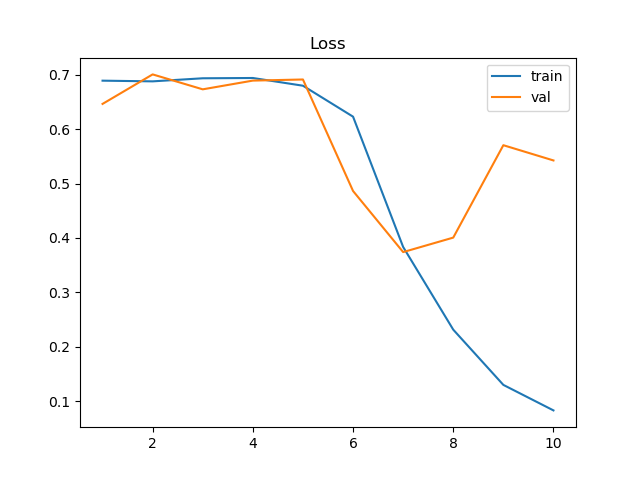
\includegraphics[width=0.6\textwidth]{../results/lstm_loss.png}
\end{figure}

\FloatBarrier

val F1:
\begin{figure}[h]
    \centering
    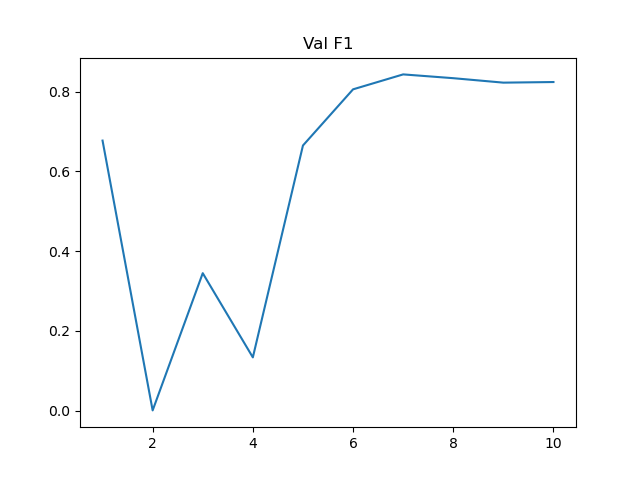
\includegraphics[width=0.6\textwidth]{../results/lstm_f1.png}
\end{figure}

\FloatBarrier

在 test set 上我们对比了单向和双向 LSTM 的结果:
在test set上的表现为:

\begin{table}[H]
    \centering
    \begin{tabular}{|c|c|c|}
        \hline 
        {\bf 指标} & {\bf 单向LSTM} & {\bf 双向LSTM}\\
        \hline
        Loss & 0.7289 & 0.4461\\
        \hline 
        Accuracy & 0.8347 & 0.8049\\
        \hline
        F1 & 0.8338 & 0.7966 \\
        \hline
    \end{tabular}
\end{table}

\begin{itemize}
    \item 双向 LSTM 的 Loss 明显更低,说明它拟合得更充分
    \item 单向 LSTM 的 Accuracy 和 F1 更高,说明它在 test set 上泛化得更好
\end{itemize}

\section{RNN-GRU}

\subsection{数据预处理}
同上 CNN 模型的数据预处理过程。

\subsection{模型结构图}

\begin{figure}[htbp]
    \centering
    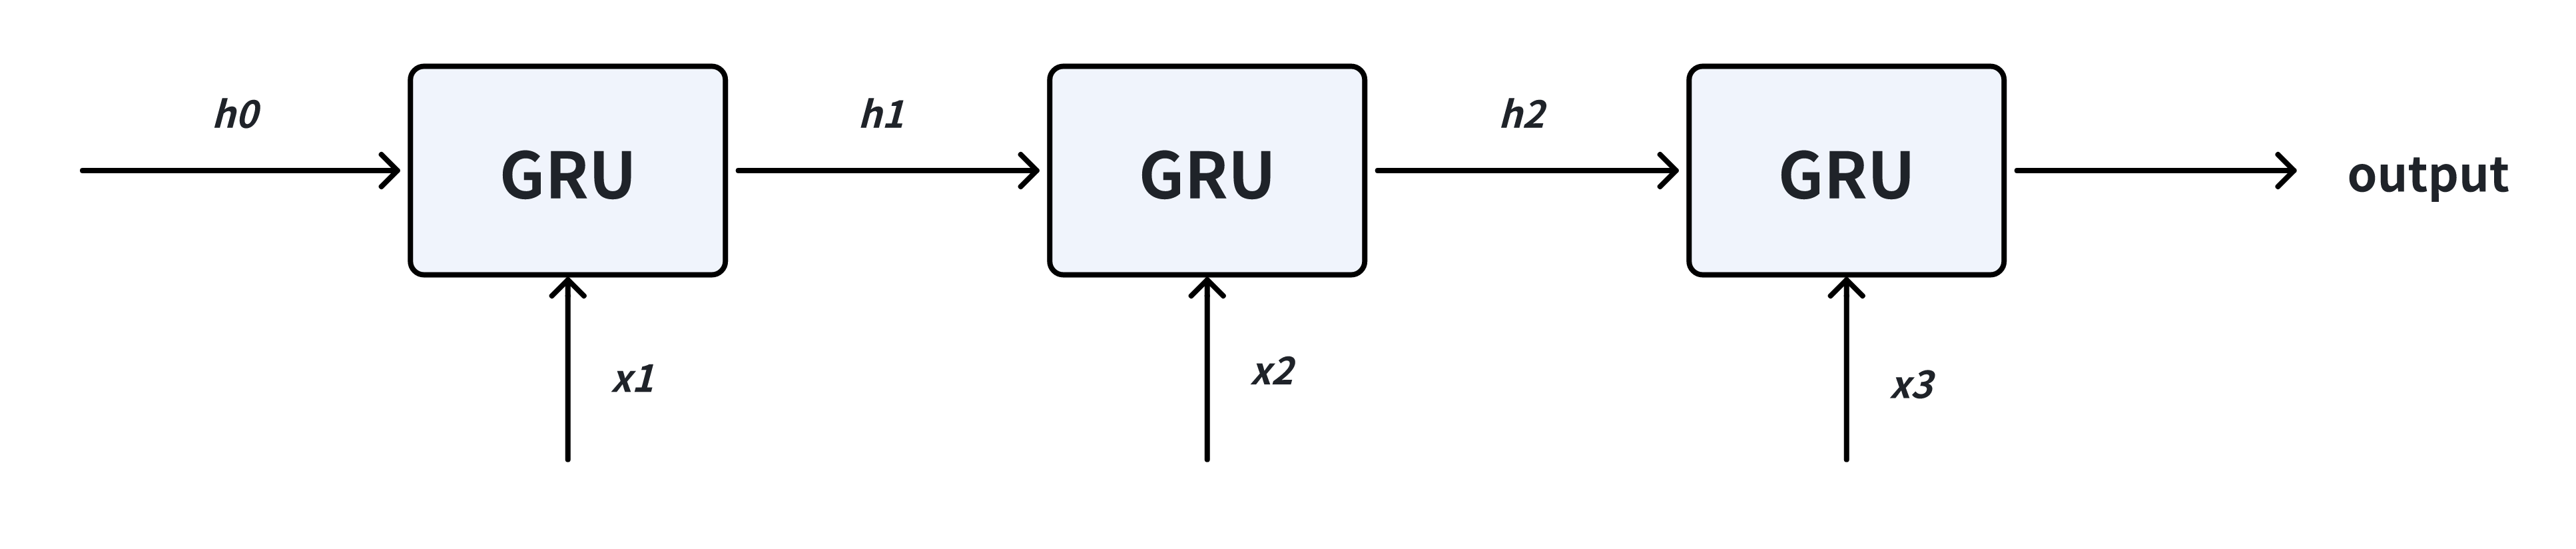
\includegraphics[width=0.6\textwidth]{img/gru.png}
\end{figure}

\FloatBarrier

\begin{figure}[htbp]
    \centering
    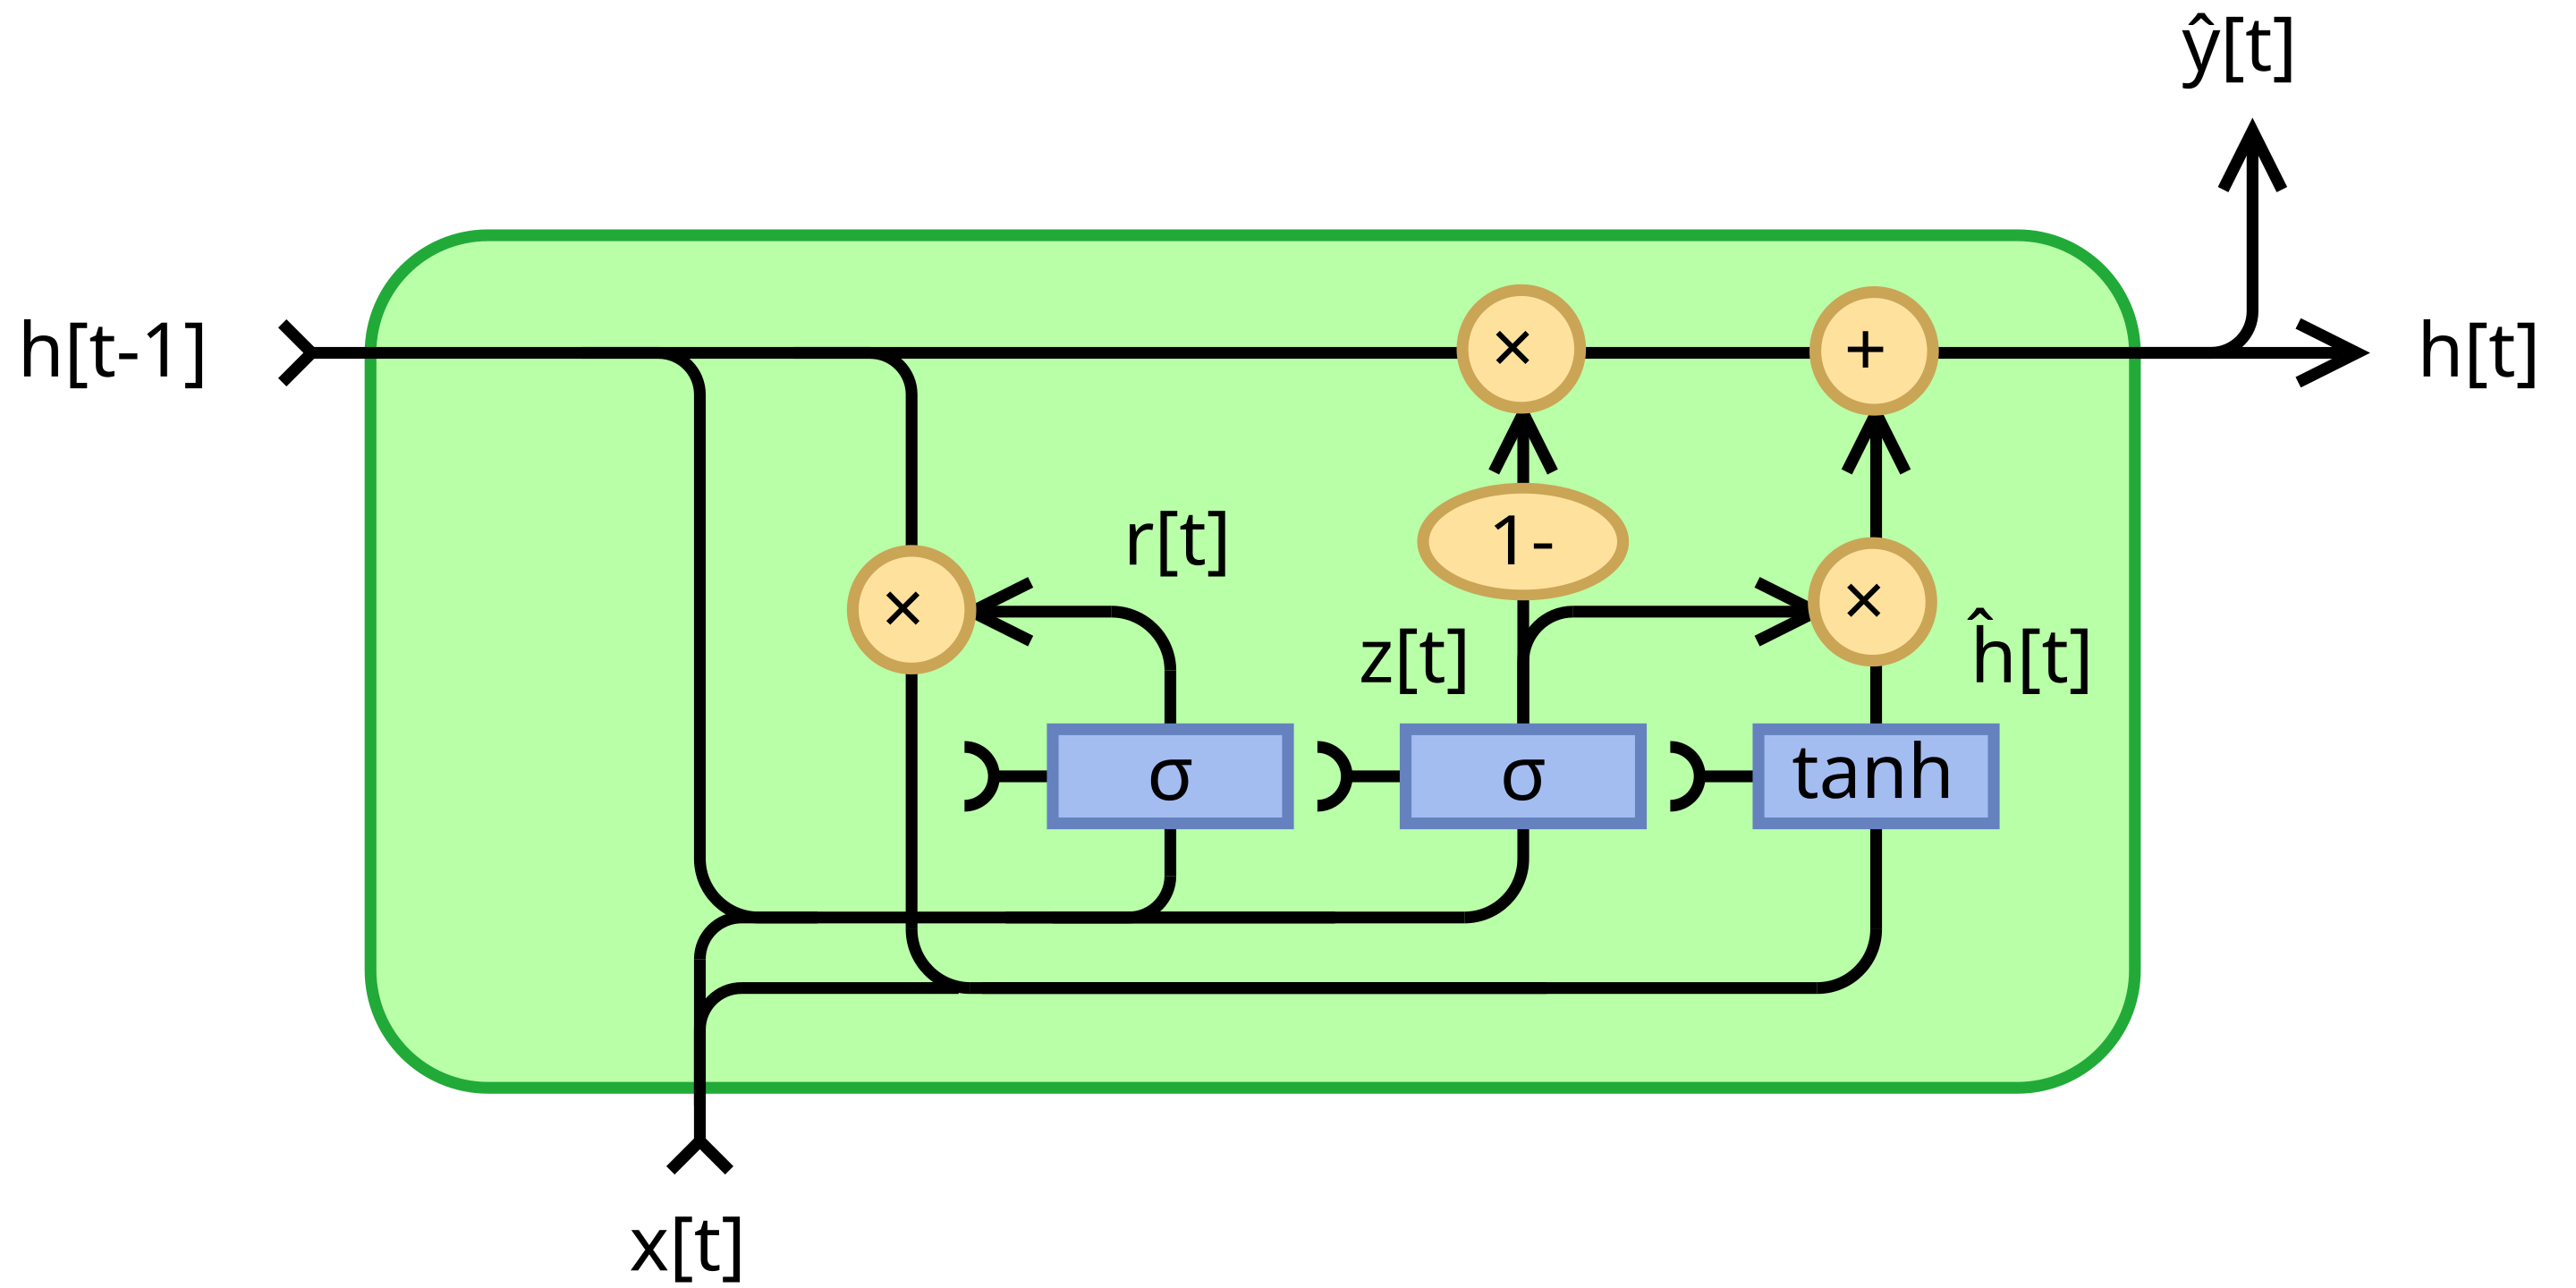
\includegraphics[width=0.6\textwidth]{img/Gated_Recurrent_Unit_base_type.svg.png}
\end{figure}

\FloatBarrier

\subsection{流程分析}
基本结构同LSTM, 但是 GRU 只有 2 个门:

\begin{itemize}
    \item 重置门: 控制当前收入和之前记忆的结合程度
    \item 更新门:控制保留多少过去信息,约等于遗忘门 + 输入门的组合
\end{itemize}

输出状态只有 $h_t$,没有记忆状态 $c_t$

\subsection{实验结果}
超参数如下:

\begin{table}[H]  
    \centering        
    \begin{tabular}{|c|c|}
    \hline
    {\bf 超参数} & {\bf 数值} \\
    \hline
    epoch & 10  \\
    \hline
    batch\_size & 128  \\
    \hline
    learning\_rate & 2e-3  \\
    \hline
    hidden\_size & 128 \\
    \hline
    num\_layers & 1 \\
    \hline
    max\_len & 60 \\
    \hline
    \end{tabular}
\end{table}

train、val accuracy:
\begin{figure}[h]
    \centering
    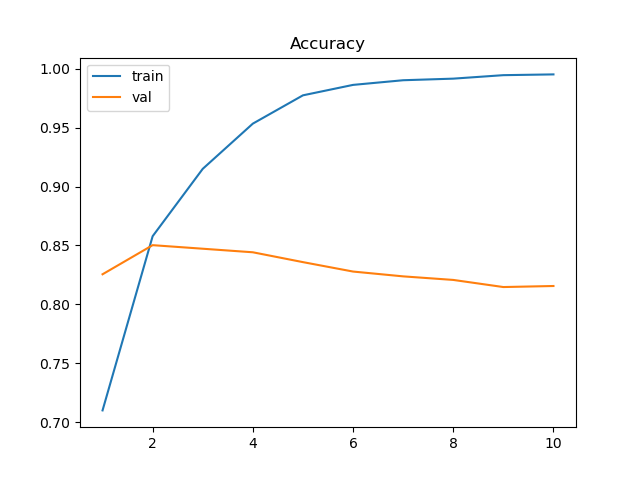
\includegraphics[width=0.6\textwidth]{../results/gru_acc.png}
\end{figure}

\FloatBarrier

train、val loss:
\begin{figure}[h]
    \centering
    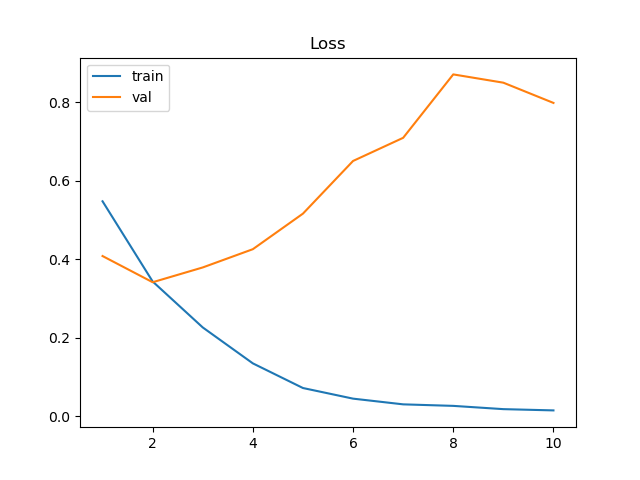
\includegraphics[width=0.6\textwidth]{../results/gru_loss.png}
\end{figure}

\FloatBarrier

val F1:
\begin{figure}[htbp]
    \centering
    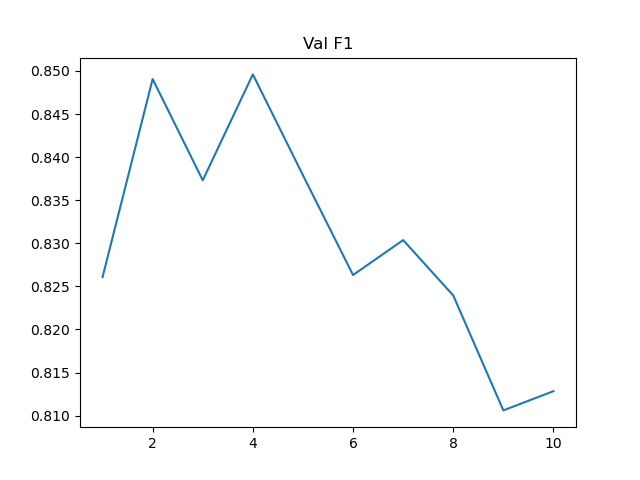
\includegraphics[width=0.6\textwidth]{../results/gru_f1.png}
\end{figure}

\FloatBarrier

在test set上的表现为:

\begin{table}[H]
    \centering
    \begin{tabular}{|c|c|}
        \hline 
        {\bf 指标} & {\bf 数值} \\
        \hline
        Loss & 0.7148 \\
        \hline 
        Accuracy & 0.8347 \\
        \hline
        F1 & 0.8365 \\
        \hline
    \end{tabular}
\end{table}

\section{BERT}

\subsection{数据预处理}

把数据集变成 HuggingFace BERT 能接受的 input\_ids , attention\_mask , labels 三张张量:

\begin{itemize}
    \item input\_ids: 句子每个 token 的词 id 组成的tensor。长度过长截断, 否则填充为0
    \item attention\_mask: 有效位置标注 1, 填充位置标注 0
    \item labels: 句子的标签
\end{itemize}

然后直接返回 PyTorch DataLoader, 可直接用于训练和验证阶段。

\subsection{模型结构图}

\begin{figure}[htbp]
    \centering
    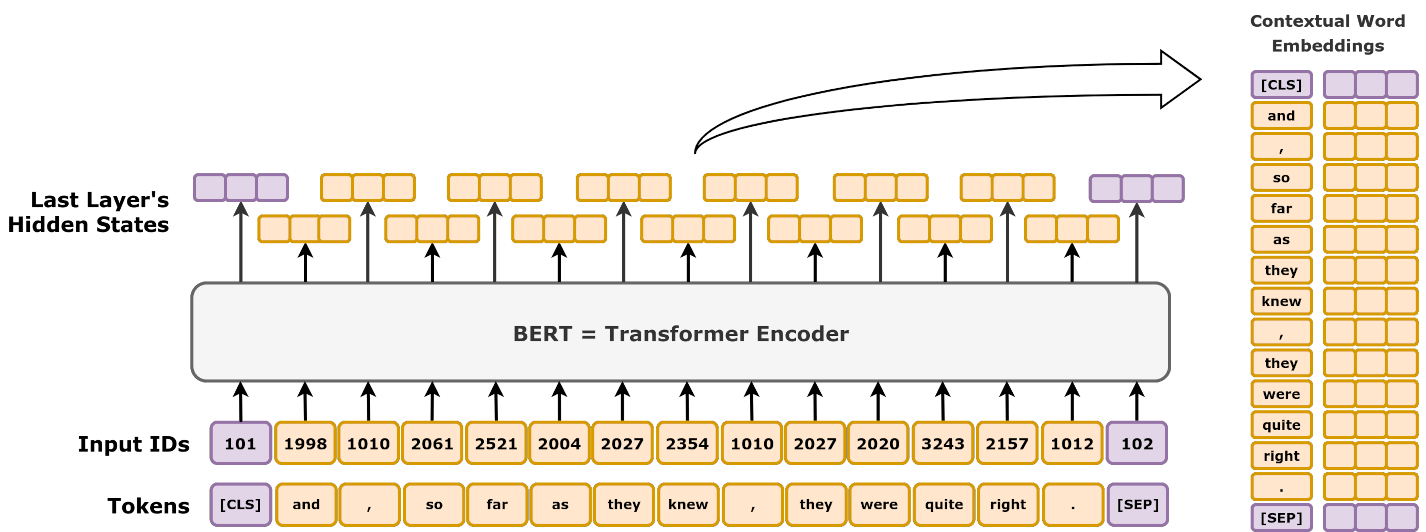
\includegraphics[width=0.6\textwidth]{img/bert.png}
\end{figure}

\FloatBarrier



\subsection{流程分析}

\begin{itemize}
    \item 从 HuggingFace 模型库加载预训练的bert模型
    \item 将预处理的数据传入模型
    \item 取 [CLS] 表示向量,代表整个句子的聚合向量,代表句子级语义
    \item cls 送入分类器,经过 Dropout + Linear
    \item Softmax后输出
\end{itemize}

\subsection{实验结果}
考虑到性能问题,本实验转移到另一台电脑的RTX4080上完成。
超参数如下:

\begin{table}[H]  
    \centering        
    \begin{tabular}{|c|c|}
    \hline
    {\bf 超参数} & {\bf 数值} \\
    \hline
    epoch & 10  \\
    \hline
    batch\_size & 16  \\
    \hline
    learning\_rate & 2e-5 \\
    \hline
    max\_len & 128 \\
    \hline
    dropout & 0.3 \\
    \hline 
    \end{tabular}
\end{table}

train、val accuracy:
\begin{figure}[h]
    \centering
    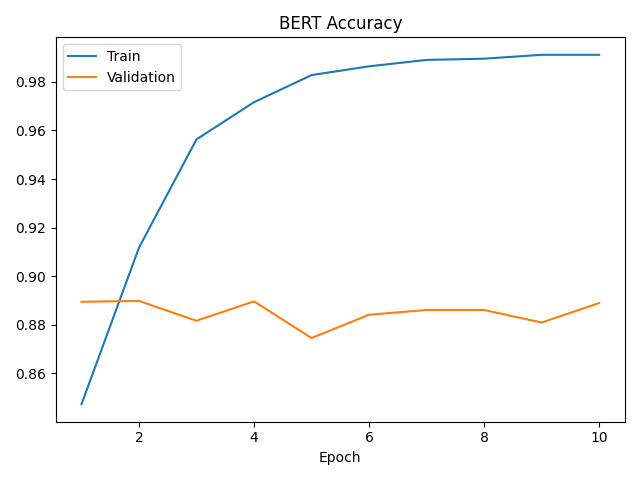
\includegraphics[width=0.6\textwidth]{../results/bert_acc.png}
\end{figure}

\FloatBarrier

train、val loss:
\begin{figure}[h]
    \centering
    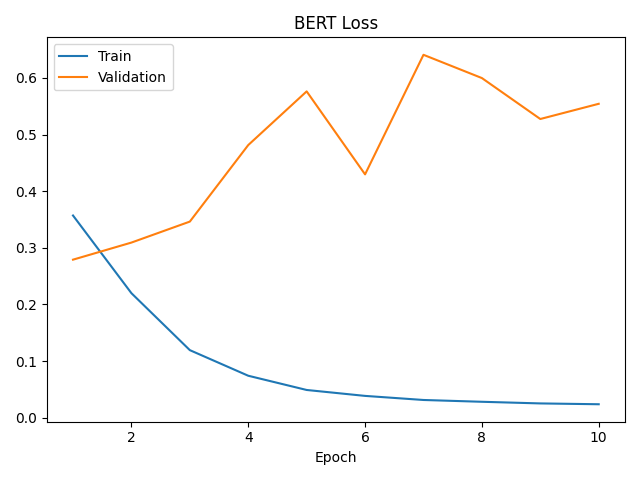
\includegraphics[width=0.6\textwidth]{../results/bert_loss.png}
\end{figure}

\FloatBarrier

val F1:
\begin{figure}[htbp]
    \centering
    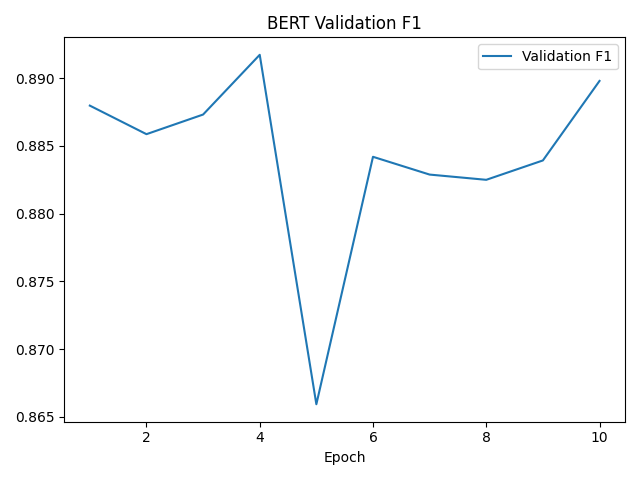
\includegraphics[width=0.6\textwidth]{../results/bert_f1.png}
\end{figure}

\FloatBarrier

在test set上的表现为:

\begin{table}[H]
    \centering
    \begin{tabular}{|c|c|}
        \hline 
        {\bf 指标} & {\bf 数值} \\
        \hline
        Loss & 0.5215 \\
        \hline 
        Accuracy & 0.8943 \\
        \hline
        F1 & 0.8966 \\
        \hline
    \end{tabular}
\end{table}

可以看到 Bert 模型的F1和Accuracy都接近了 0.9, 与前面的模型相比有极大提升。

\section{Baseline: MLP}

\subsection{数据预处理}
同上过程。

\subsection{模型结构图}

\begin{center}
    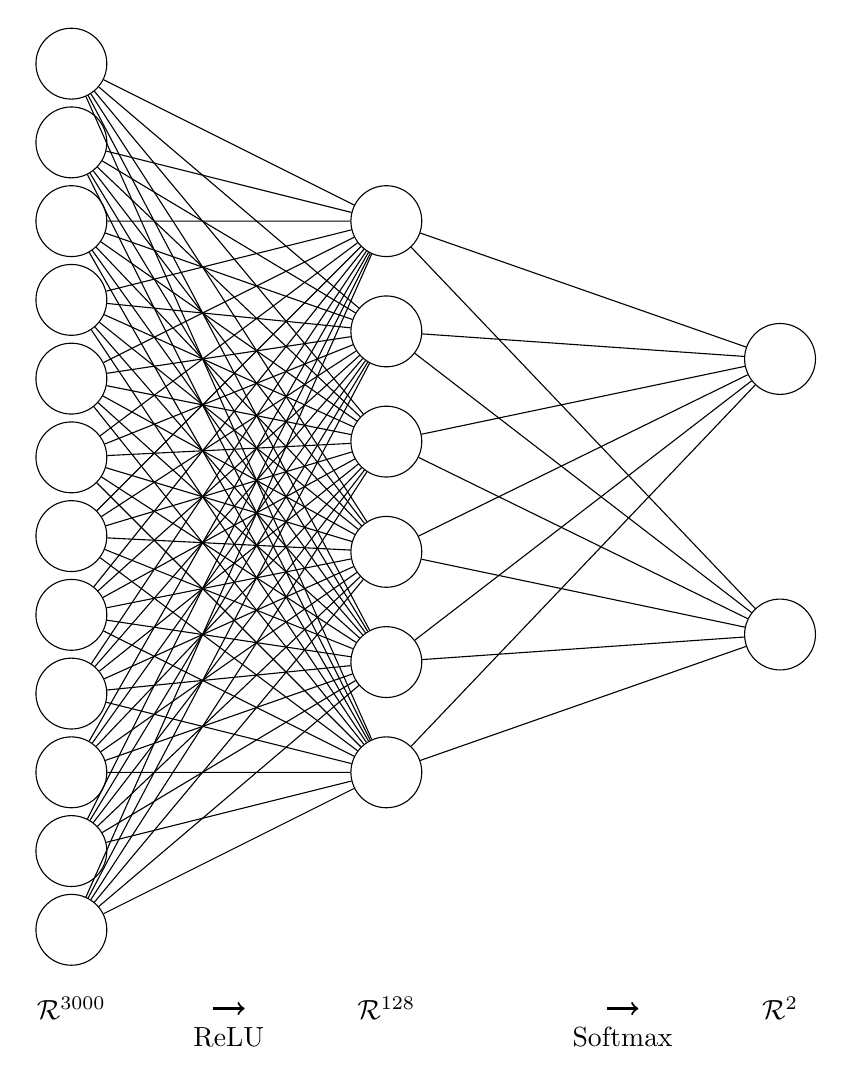
\begin{tikzpicture}[
        neuron/.style={circle, draw=black, minimum size=9mm},
        every label/.style={font=\scriptsize},
        font=\normalsize
    ]
    
    % ---------- 层参数 ----------
    \def\inputnum{12}
    \def\hiddennum{6}
    \def\outputnum{2}
    
    \def\inputgap{1.0}
    \def\hiddengap{1.4}
    \def\outputgap{3.5}
    
    % ---------- 输入层 ----------
    \foreach \i in {1,...,\inputnum} {
        \pgfmathsetmacro\y{(\inputnum-1)*\inputgap/2 - (\i-1)*\inputgap}
        \node[neuron] (I\i) at (0, \y) {};
    }
    
    % ---------- 隐藏层 ----------
    \foreach \i in {1,...,\hiddennum} {
        \pgfmathsetmacro\y{(\hiddennum-1)*\hiddengap/2 - (\i-1)*\hiddengap}
        \node[neuron] (H\i) at (4, \y) {};
    }
    
    % ---------- 输出层 ----------
    \foreach \i in {1,...,\outputnum} {
        \pgfmathsetmacro\y{(\outputnum-1)*\outputgap/2 - (\i-1)*\outputgap}
        \node[neuron] (O\i) at (9, \y) {};
    }
    
    % ---------- 连线 ----------
    \foreach \i in {1,...,\inputnum} {
        \foreach \j in {1,...,\hiddennum} {
            \draw[thin] (I\i) -- (H\j);
        }
    }
    
    \foreach \i in {1,...,\hiddennum} {
        \foreach \j in {1,...,\outputnum} {
            \draw[thin] (H\i) -- (O\j);
        }
    }
    
    % ---------- 层标签 ----------
    \node at (0, -6.5) {$\mathcal{R}^{3000}$};
    \node at (4, -6.5) {$\mathcal{R}^{128}$};
    \node at (9, -6.5) {$\mathcal{R}^{2}$};
    
    % ---------- 激活函数箭头 ----------
    \draw[->, thick] (1.8, -6.5) -- (2.2, -6.5) node[midway, below=3pt] {ReLU};
    \draw[->, thick] (6.8, -6.5) -- (7.2, -6.5) node[midway, below=3pt] {Softmax};
    
    \end{tikzpicture}
    \end{center}
\subsection{流程分析}

\begin{itemize}
    \item 使用 max\_len $\times $ 50 规模的输入,映射到 hidden\_size 规模的隐藏层
    \item ReLU + Dropout
    \item 将隐藏层特征映射为 2 个神经元
    \item Softmax, 输出结果
\end{itemize}

\subsection{实验结果}

超参数如下:

\begin{table}[H]  
    \centering        
    \begin{tabular}{|c|c|}
    \hline
    {\bf 超参数} & {\bf 数值} \\
    \hline
    epoch & 10  \\
    \hline
    batch\_size & 128  \\
    \hline
    learning\_rate & 2e-3  \\
    \hline
    hidden\_size & 128 \\
    \hline
    max\_len & 60 \\
    \hline
    \end{tabular}
\end{table}

train、val accuracy:
\begin{figure}[h]
    \centering
    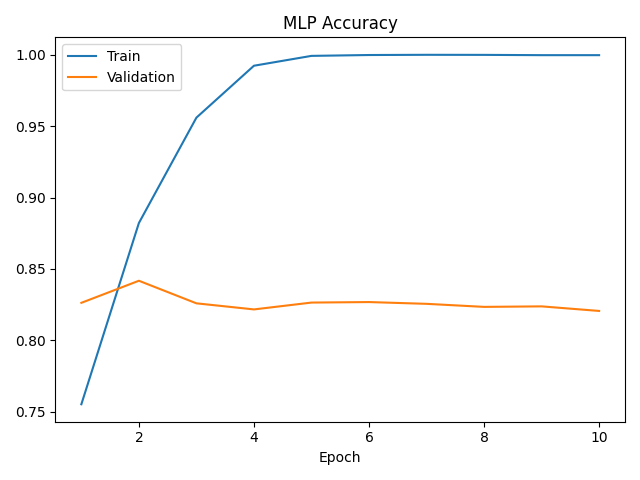
\includegraphics[width=0.6\textwidth]{../results/mlp_acc.png}
\end{figure}

\FloatBarrier

train、val loss:
\begin{figure}[h]
    \centering
    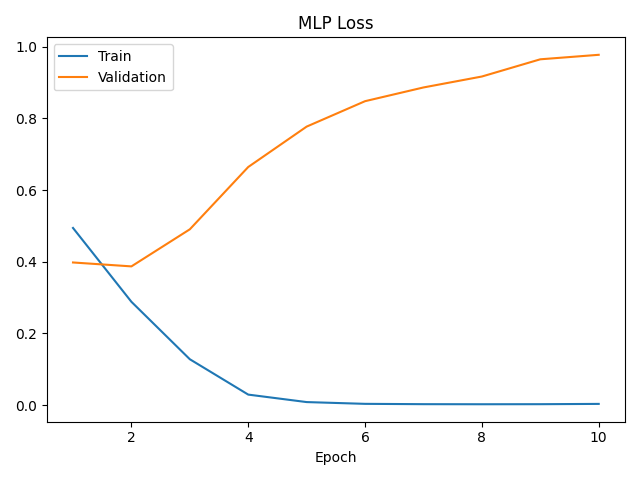
\includegraphics[width=0.6\textwidth]{../results/mlp_loss.png}
\end{figure}

\FloatBarrier

val F1:
\begin{figure}[htbp]
    \centering
    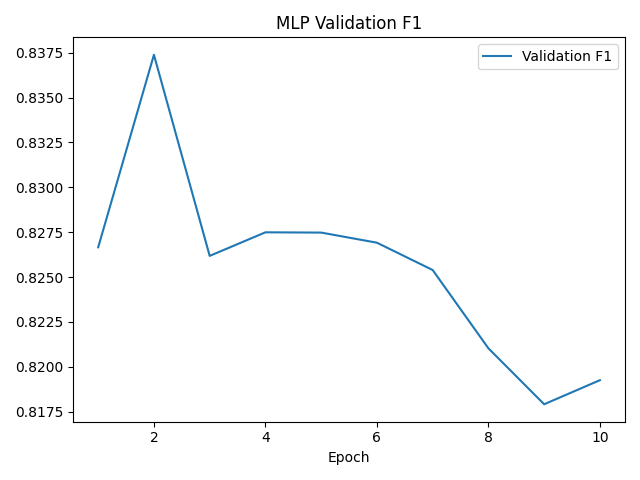
\includegraphics[width=0.6\textwidth]{../results/mlp_f1.png}
\end{figure}

\FloatBarrier

在test set上的表现为:

\begin{table}[H]
    \centering
    \begin{tabular}{|c|c|}
        \hline 
        {\bf 指标} & {\bf 数值} \\
        \hline
        Loss & 0.9975 \\
        \hline 
        Accuracy & 0.8049 \\
        \hline
        F1 & 0.7931 \\
        \hline
    \end{tabular}
\end{table}

值得注意的是训练到第 10 轮的时候, train set 的accuracy已经几乎完全接近1了。

\section{参数效果对比}

\subsection{batch size 实验}

\begin{figure}[h]
    \centering
    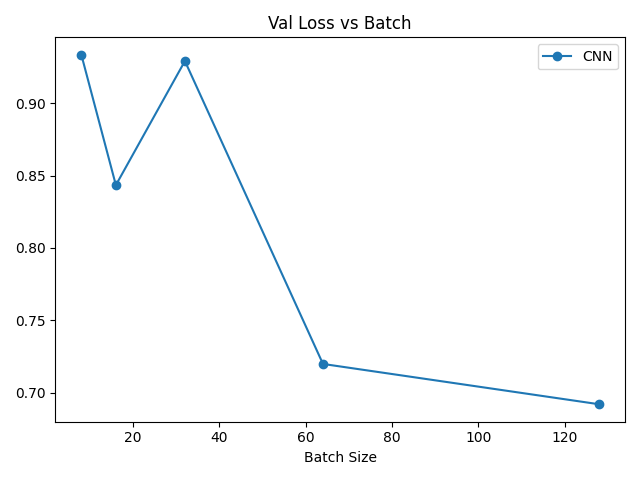
\includegraphics[width=0.6\textwidth]{../results/batch_loss.png}
    \caption{不同batch的loss表现}
\end{figure}

\begin{figure}[h]
    \centering
    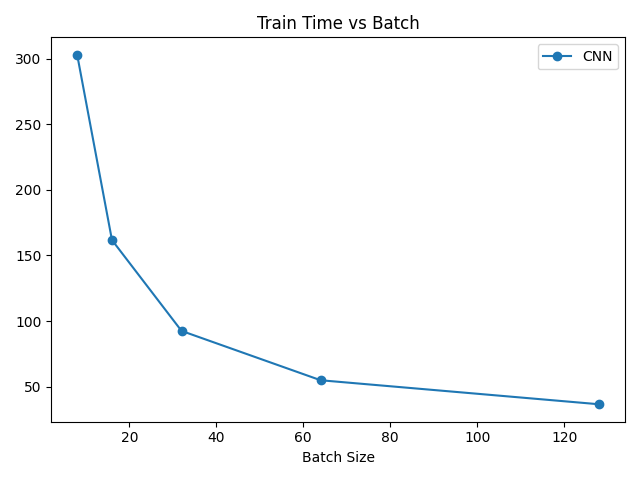
\includegraphics[width=0.6\textwidth]{../results/batch_time.png}
    \caption{不同batch的用时表现}
\end{figure}

当选取的 batch size 越大,意味着反向传播过程的进行次数越少,这也就对应着训
练时长的降低。随着 batch\_size 增大,模型更新更稳定、更接近“真实梯度方向”,训练过程变得平滑,这通常有助于更好的收敛,因此 valid loss 在一定范围内可能会减小。
但这不是绝对的趋势 —— 它受到多因素影响。 CNN 本身模型参数量小 → 更依赖稳定训练
TextCNN 这种模型,参数少、结构浅,训练非常敏感。小 batch 容易抖动,训练过程不稳定,valid loss 高。
大 batch 给它更稳定的梯度,反而容易学得好。
\end{document}